This document describes how to get started with the CaesarJ Development Tools in Eclipse. CJDT provides a rich set of features for working with Caesar programs inside Eclipse.\\\\
\subsection{CJDT Highlights:}
\begin{itemize}
	\item Editor support with keyword highlighting\\\\
	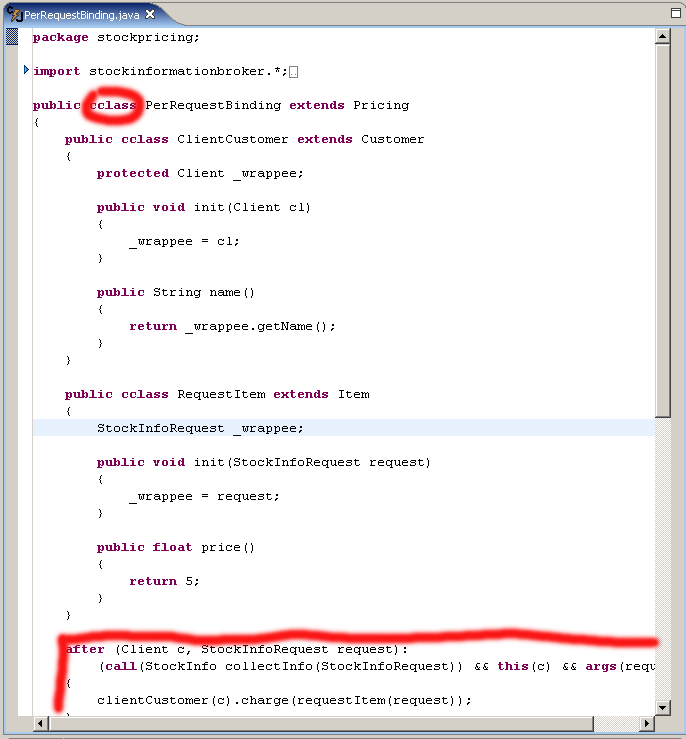
\includegraphics[width=0.95\textwidth]{images/hilight.png}\\

  \item Outline view showing structural members and crosscutting relationships (e.g. from an advice declaration to
     the places it advises).\\\\
  \textbf{TODO BILD GEHT NICHT RICHTIG ASPECTE FEHLEN}\\
  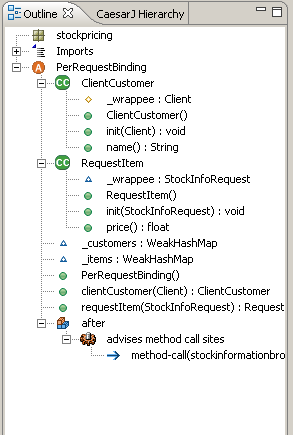
\includegraphics[width=0.30\textwidth]{images/outline.png}\\
     
  \item Caesar-Hierarchy\\\\
	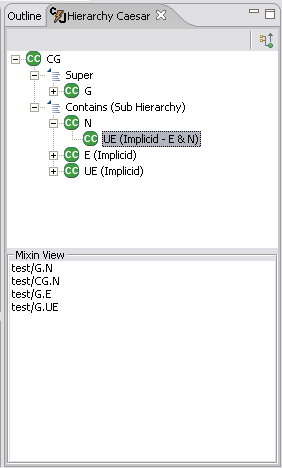
\includegraphics[width=0.30\textwidth]{images/hierarchy.png}\newpage

     
  \item New Caesar Project wizard\\\\
  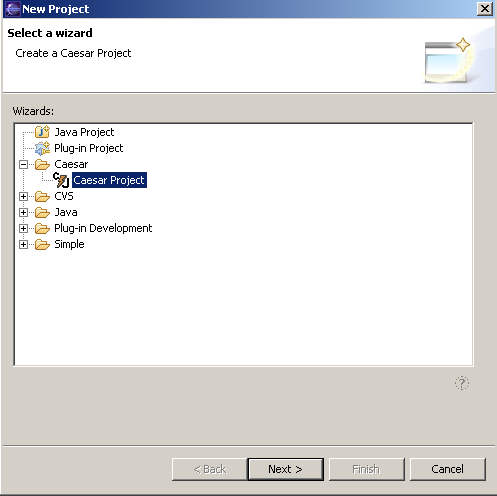
\includegraphics[width=0.60\textwidth]{images/project_wizard.png}\\

  \item Debugging support\\\\
	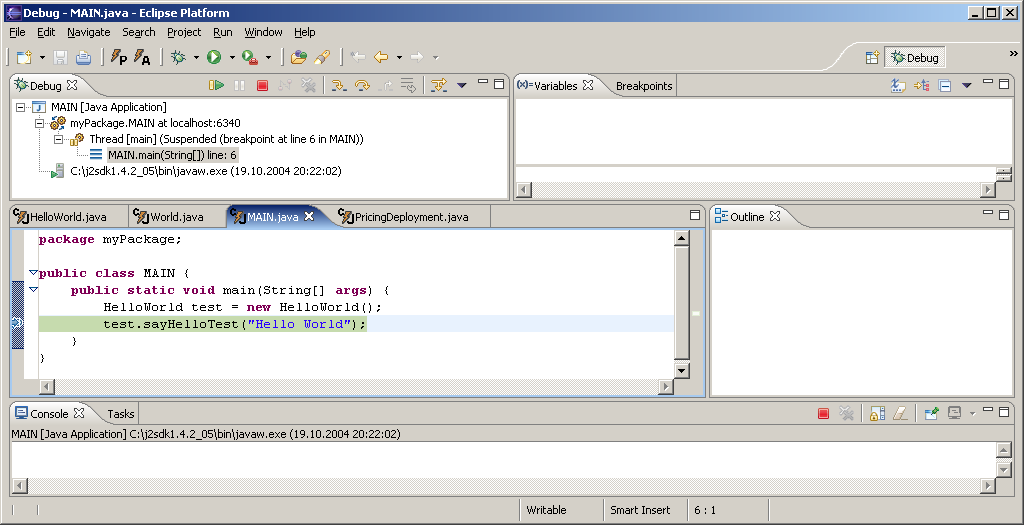
\includegraphics[width=0.95\textwidth]{images/debug1.png}\\
\end{itemize}